\documentclass[10pt, handout]{beamer}
\usepackage{xmpincl}
\includexmp{license}
\usepackage[T1]{fontenc}
\usepackage[latin1]{inputenc}
\usepackage{ae}
\usepackage[french]{babel}
\usepackage{array, longtable}
\usetheme{Antibes}
\setbeamertemplate{navigation symbols}{}

% for printing
\usepackage{pgfpages}
\pgfpagesuselayout{2 on 1}[a4paper,border shrink=5mm]
%\pgfpagesuselayout{resize to}[a4paper,border shrink=5mm,landscape]


\usepackage{listings}
\usepackage{verbatim}
\makeatletter
\newwrite\lstvrb@out
\newenvironment{code}{%
  \begingroup
  \@bsphack
  \immediate\openout\lstvrb@out\jobname.lst
  \let\do\@makeother\dospecials\catcode`\^^M\active
  \def\verbatim@processline{%
    \immediate\write\lstvrb@out{\the\verbatim@line}}%
  \verbatim@start}{%
  \immediate\closeout\lstvrb@out
  \@esphack
  \endgroup

  \begin{alertblock}{}
    \lstinputlisting[language=java]{\jobname.lst}
  \end{alertblock}}
\makeatother

\lstset{language=java, basicstyle=\small, commentstyle=\color{blue}\textrm}

\title{Computer Science Introductory Course MSc - Introduction to Java}

\subtitle{Lecture 1: Diving into java}

\author[Pablo Oliveira]{Pablo Oliveira \texttt{<pablo@sifflez.org>}}
\institute{T\'el\'ecom ParisTech}

\date{}

\begin{document}
\begin{frame}
  \titlepage
\end{frame}

\begin{frame}
  \frametitle{Outline}
  \tableofcontents
\end{frame}

\section{Introduction}
\begin{frame}[fragile]
  \frametitle{Introduction: Execution model}
  \begin{itemize}
    \item Java programs run inside a Virtual Machine (JVM), "a software implementation" of a computer
          (making Java programs portable among different architectures).
    \item For the sake of performance and space, the JVM reads bytecode (a low level language).
    \item It is easier for humans to write programs in a more expressive, high level language, like Java.
    \item The Java compiler is an automatic translator from Java to Bytecode.
  \end{itemize}
\end{frame}

\begin{frame}[fragile]
  \frametitle{Introduction: Concepts}
  \begin{itemize}
   \item A computer program can be seen as a transformation from a state of a computer to a new one.
   \item So very informally, programming is a matter of transforming data:
    \begin{itemize}
      \item Find a computer representation of data
      \item Write methods to transform this data
    \end{itemize}
   \item In this lecture we will learn about:
  \end{itemize}
   \begin{description}
      \item[primitive types:] Basic representations of data.
      \item[      operators:] Simple operations on data.
      \item[        classes:] Combine data representation and methods to transform data.
      \item[   control flow:] Control which operations are done and how many times.
   \end{description}
\end{frame}

\section{Primitive types}

\begin{frame}
  \frametitle{Outline}
  \tableofcontents[currentsection]
\end{frame}

\begin{frame}[fragile]
  \frametitle{Representing data}
  Data is encoded in memory as a binary string.
  \begin{code}
  bin: 00000000 01001000 00000000 01101001
  dec: 0        72       0        105
  \end{code}
  \structure{What does this value represent ?}
  \pause
  \begin{example}
    \begin{description}
    \item[2d line]: (0,72) to (0,105)
      \pause
      \item[integer]: 4718697
      \pause
    \item[float]: 6.612303E-39 (IEEE 754)
      \pause
      \item[string]: 'H' 'i'
      \pause
      \item[...]
    \end{description}
  \end{example}
\end{frame}

% emphasize that = is different than equality
\begin{frame}[fragile]
  \frametitle{Variables and Types}
  \begin{itemize}
  \item
  To lift this ambiguity we introduce \structure{types},
  which specify how a value should be used.
  \item
  We also give each value a name (should start with \{letter, \$, \_ \} and contain only \{alphanumeric, \$, \_\}).
  \item
  We call the association (name, type, value) a variable.
  \end{itemize}

  \begin{example}
   \begin{longtable}{l|r}
   \lstinline!boolean is_it_raining = true;! & 1 bit logic value\\
   \pause
   \lstinline!byte life_expectancy = 70;! & 8 bit range $[-128..127]$ \\
   \lstinline!short year;! & 16 bit defined on $[-2^{15}..2^{15}-1]$ \\
   \lstinline!char unicode_character = 'A';! & UTF-16 caracter \\
   \pause
   \lstinline!int city_population = 2167994;! & 32 bit range $[-2^{31}..2^{31}-1]$ \\
   \pause
   \lstinline!long molecules;! &  64 bit range $[-2^{63}..2^{63}-1]$ \\
   \hline
   \pause
   \lstinline!float mean_grade = 13.54;! & single precision(ex. 8 mt. 23) \\
   \lstinline!double angular_speed;! & double precision(ex. 11 mt. 52) \\
  \end{longtable}
\end{example}
\end{frame}


% maybe introduce scopes before XXX
\begin{frame}[fragile]
  \frametitle{Mutable variables, assignment, final variables}

  The value of a variable can be modified during the execution of a program,
  except for final variables (which can only be assigned once).

  \begin{code}
int a; // variable declaration
float b = 3; /* variable declaration with
                initial assignment */
final float pi;
pi = 3.14159;

a = 8;  // assignment
b = 1;  // assignment
pi = 0; // illegal (won't compile)
  \end{code}
\end{frame}

\begin{frame}[fragile]
  \frametitle{Arrays}
  Arrays model a contiguous, random access, fixed-length, \structure{collection of values}.
  The values of an array are of the same type.

  \begin{code}
// The type of the array price is float[]
float[] price;

// reserve memory for 3 elements
price = new float[3];

// initialize the values of the elements
price[0] = 1.00;
price[1] = 5.99;
price[2] = 3.25;

// Syntax sugar for this is:
float[] price = {1.00, 5.99, 3.25};
  \end{code}
\end{frame}

\begin{frame}[fragile]
  \frametitle{Strings}
  Strings represent a collection of characters.
  \begin{code}
    String message = "Hello World";
  \end{code}

  \begin{alertblock}{Caution}
    \begin{itemize}
    \item Strings and arrays are a mix between objects and primitive types and thus some care must be taken when manipulating them.
    \item In the next lecture we will explain why when we'll talk about references and immutability.
    \end{itemize}
  \end{alertblock}
\end{frame}


\section{Operators}

\begin{frame}
  \frametitle{Outline}
  \tableofcontents[currentsection]
\end{frame}


\begin{frame}[fragile]
  \frametitle{Simple Operators}
  \begin{itemize}
  \item
  Operators are special symbols which perform an operation on some operands.
  \item
  The semantic of the operator depends on the type of the operands.
  \end{itemize}

  \begin{example}
   \begin{longtable}{l|r}
   \lstinline!a = 5; b[4] = 30!& assignment\\
   \pause
   \lstinline!5 + 4! $\rightarrow$ \lstinline!9! & sum \\
   \lstinline!5 - 4! $\rightarrow$ \lstinline!1! & substraction \\
   \pause
   \lstinline!"hello " + "world"! $\rightarrow$ \lstinline!"hello world"! & concatenation \\
   \pause
   \lstinline!4 * 4! $\rightarrow$ \lstinline!16! & multiplication \\
   \lstinline!15 / 2! $\rightarrow$ \lstinline!7!,
   \lstinline!15.0 / 2! $\rightarrow$ \lstinline!7.5! & integer or float division \\
   \lstinline!15 % 2! $\rightarrow$ \lstinline!1! & modulo \\
   \pause
   \lstinline!15 > 12! $\rightarrow$ \lstinline!true! & bigger than \\
   \lstinline!< >= <=! & other comparison operators \\
  \end{longtable}
  \end{example}
\end{frame}


% hard to understand
\begin{frame}[fragile]
  \frametitle{Increment operators}
  \begin{itemize}
  \item \structure{Increment (\lstinline!++!), decrement (\lstinline!--!)  operators:}
 \begin{code}
    int a,b,c;

    a = 42;
    b = a++;
    \\here b evaluates to 42 and a to 43

    a = 42;
    b = ++a;
    \\here b evaluates to 43 and a to 43
  \end{code}
  \item with \lstinline!++a! the value of a is incremented, then the right side of the assignment is evaluated.
  \item with \lstinline!a++! the right side of the assignment is evaluated, then a is incremented.

\end{itemize}
\end{frame}

\begin{frame}[fragile]
  \frametitle{More Operators}
  \begin{itemize}
  \item Operation + assignment (\lstinline!+= -= *= /=! etc ...)
  \begin{code}
     a += b;    // equivalent to:
     a = a + b;
  \end{code}
  \item Equality \lstinline@==@ and Inequality \lstinline@!=@
  \begin{code}
    int a, b;
    a = 5;
    c = 2;
    b = c + 3;
    a == b; // --> true
    a != c; // --> true
  \end{code}
  \item \alert{Referential equality when used with objects, strings and arrays (we'll come back to this later)}
  \end{itemize}
\end{frame}

\begin{frame}[fragile]
  \frametitle{Boolean operators}
  \begin{itemize}
    \item Boolean Operators
    \begin{code}
      bool a = false;
      bool b = true;

      /* not */     !a // --> true
      /* and */     a && b // --> false
      /* or */      a || b // --> true

      /* Careful: Lazy */
      int a = 0;
      (false) && (a++ > 0) // a evaluates to 0
      (true)  || (a++ > 0) // a evaluates to 0
    \end{code}
  \end{itemize}
\end{frame}

\begin{frame}[fragile]
  \frametitle{Other operators}
  \begin{itemize}
    \item Ternary Operator (\lstinline!condition?true_stm:false_stm!)  ex: \lstinline!(a>b) ? a : b!
    \item Bitwise Operators (\lstinline!>> << >>> & |!)
    \item \lstinline!instanceof!
    \end{itemize}
\end{frame}

\section{Basic OOP}
\begin{frame}
  \frametitle{Outline}
  \tableofcontents[currentsection]
\end{frame}

\begin{frame}[fragile]
  \frametitle{Objects}
  \begin{definition}
    An \structure{object} is the association of:
    \begin{itemize}
      \item a State (i.e. data)
      \item some Methods (i.e. operations that change/read state)
    \end{itemize}
  \end{definition}
  \pause
\begin{example}
  A \alert{turtle} has a state composed of \alert{its color, its position and its orientation},
  and some methods: \alert{turn, advance and readPosition}.
  \begin{center}
  \only<2-3>{
  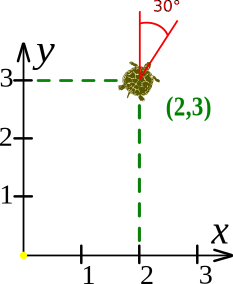
\includegraphics[height=3cm]{tortue}
  }
  \only<3>{
  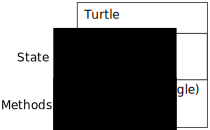
\includegraphics[height=3cm]{car1}
  }
  \end{center}

\end{example}
\end{frame}

\begin{frame}
  \frametitle{Classes}
  \only<1| handout:1>{
  \begin{Definition}
    A \structure{class} is a blueprint for making objects. A class defines the common attributes
    of a family of objects:
      \begin{itemize}
        \item the methods they share
        \item the types of variables they have
      \end{itemize}
  \end{Definition}
  }
  \only<2-3| handout:2-3>{
  \begin{Example}
    \begin{center}
    \only<2| handout:2>{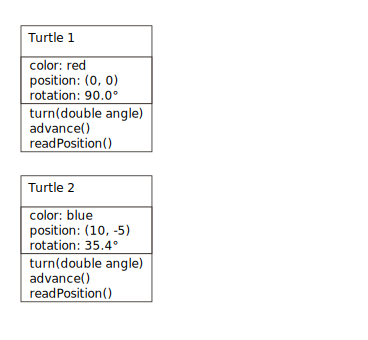
\includegraphics[height=7cm]{car2}}
    \only<3| handout:3>{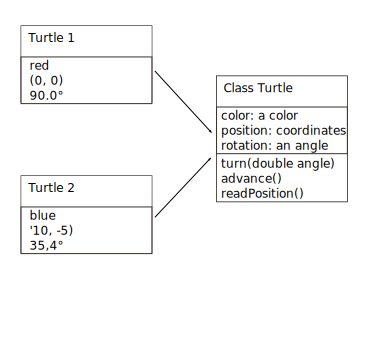
\includegraphics[height=7cm]{car3}}
    \end{center}
  \end{Example}
  }
\end{frame}

\begin{frame}[fragile]
  \frametitle{Anatomy of a method}
  \begin{center}
  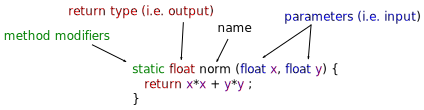
\includegraphics[width=\linewidth]{method_anatomy}
  \end{center}
\end{frame}


\begin{frame}[fragile,shrink]
  \frametitle{In Java}
  \begin{code}
class Turtle {
  Color color;
  Position position;
  double rotation;

  void turn(double angle) { rotation += angle; }
  void advance() {
    int step_size = 5;
    position.x += step_size * cos(rotation*Math.PI/180);
    position.y += step_size * sin(rotation*Math.PI/180);
  }

  Position readPosition() {
    return position;
  }
}
  \end{code}
  \pause
  \begin{code}
Turtle turtle1 = new Turtle();
Turtle turtle2 = new Turtle();

Position pos = turtle1.readPosition();
turtle2.turn(20); turtle2.advance();
  \end{code}
\end{frame}

\begin{frame}[fragile]
  \frametitle{Instance Methods/Variables}
  \begin{itemize}
  \item Objects turtle1 and turtle2 are called \alert{instances or objects} of class Turtle,
  \item \lstinline!turtle2.color! represents the color \structure{for the specific instance turtle2}:
    \newline $\rightarrow$ \alert{color is an instance variable}
  \item \lstinline!turtle1.readPosition()! returns the position of \structure{the specific instance turtle1}:
    \newline $\rightarrow$ \alert{readPosition() is an instance method}
  \end{itemize}

  \begin{definition}
    An instance method or instance variable is only relevant in the context of a particular object.
  \end{definition}
\end{frame}

\begin{frame}[fragile,shrink]
  \frametitle{Static Methods/Variables}
    \structure{Q: how to share a common variable between all the objects in a class ?}
    \begin{code}
class Turtle {
  static int step_size = 5;
}
    \end{code}
    \pause
    \structure{Q: how to write a method independent from a particular instance ?}
    \begin{code}
class Turtle {
  static double degreesToRadians(double deg) {
    return deg * Math.PI/180;
  }
}

Turtle.degreesToRadians(30); -> 1.0471975512

    \end{code}
    \pause
    \begin{definition}
      A static variable is shared among all the instances of a class.
      A static method is called in the context of a class and not for a specific instance.
      Static variables are also called class variables.
    \end{definition}
\end{frame}

\begin{frame}[fragile,shrink]
  \frametitle{Local Variables / Scope}
  \begin{definition}
    Variables defined inside a method are called local variables.

    The scope of a variable is the portion of code where it is visible (ie. where you can read it,
    or modify it).
   \end{definition}

    \begin{itemize}
      \item Local variables are only visible inside their method.
      \item Instance and Static variables are visible in all the methods from their class.
    \end{itemize}

    In the next lecture we will talk about the visibility of methods, and about access modifiers
    that regulate the visibility of methods/variables outside their class.
\end{frame}


\begin{frame}[fragile]
  \frametitle{Main: the program entry point}
  \structure{Q: (At last ...) How do we start things up ?}
  \begin{code}
    class MyFirstJavaProgram{
      public static void main (String args[]) {
        System.out.println("Hello world!");
      }
    }
  \end{code}
  (Note: public means this method can be called from anywhere, this is a prerequisite for
   the main method)
\end{frame}
%XXX anywhere ... explain better scopes

\section{Control Flow}
\begin{frame}
  \frametitle{Outline}
  \tableofcontents[currentsection]
\end{frame}

\begin{frame}[fragile]
  \frametitle{If - else}
  \structure{Depending on a predicate choose which branch to execute}
    \begin{code}
if (predicate) block1 else block2

static int collatz (int n) {
  if (n % 2 == 0) {
    return n/2;
  } else {
    return 3*n + 1;
  }
}
    \end{code}

  \structure{code between \{\} is called a block, variables defined inside a block are not visible outside}
\end{frame}

\begin{frame}[fragile]
  \frametitle{while}
  \structure{Execute a block repeatedly while a predicate is true}
  \begin{code}
while(predicate)
  block;

static int gcd(int a, int b) {
  while (b != 0) {
    int t = b;
    b = a % b;
    a = t;
  }
  return a;
}
  \end{code}
  Above if the predicate is false the block is never executed.
  When appropriate, you can use instead \lstinline!do { ... } while (predicate);! which always executes the block at least once.
\end{frame}

\begin{frame}[fragile]
  \frametitle{for}

  \structure{More sophisticated loop}

  \begin{code}
for (statement; predicate; statement)
  block

for (int i = 0; i < 100; i++) {
  System.out.println(i);
}
  \end{code}

  \structure{Syntax sugar for:}
  \begin{code}
int i = 0;
while (i < 100) {
  System.out.println(i);
  i++;
}
  \end{code}
\end{frame}

\begin{frame}[fragile]
\frametitle{break and continue}
\structure{Escaping from loops}
\begin{itemize}
   \item break will exit the loop from which it is called
   \item continue will jump to the next iteration of the loop from which it is called
\end{itemize}

\begin{code}
int whereIs(int element, int[] set) {
  int i;
  for (i = 0; i < set.length; i++) {
    if (element == set[i]) {
      break;
    }
  }
  return (i < set.length) ? i : -1;
}
\end{code}
\end{frame}

\begin{frame}[fragile]
\structure{You can also escape using return, which here avoids a test and is more elegant.}
\begin{code}
int whereIs(int element, int[] set) {
  for (int i = 0; i < set.length; i++) {
    if (element == set[i]) {
      return i;
    }
  }
  return -1;
}
\end{code}

\structure{We won't discuss switch/case control structure. If interested you may look it up! }
\end{frame}

\begin{frame}[fragile, plain]
\begin{center}
  \tiny
  This work is licensed under a Creative Commons Attribution-Noncommercial-Share Alike 3.0 Unported License.
\vtop{
  \vskip-3ex
  \hbox{
    \includegraphics[height=0.4cm]{cc-logo}
  }
}
\end{center}
\end{frame}
\end{document}
